\chapter{Referencial Teórico}

O desenvolvimento de tecnologias linguisticamente sensíveis requer um embasamento teórico que reconheça a linguagem não apenas como um sistema de signos, mas como uma prática social dinâmica e multifacetada. As perspectivas de Bakhtin sobre o dialogismo, de Paulo Freire acerca da linguagem como prática libertadora, e de Zuin sobre a comunicação rural como encontro de saberes, oferecem um arcabouço conceitual para esta investigação.

\section{A linguagem como fenômeno dialógico}
O conceito de dialogismo, conforme formulado por Mikhail Bakhtin, é central para a compreensão da linguagem em sua dimensão social e interativa. Bakhtin postula que nenhuma enunciação é um ato isolado; ao contrário, toda fala carrega em si o eco de outras vozes e se constitui na interação com elas \cite{bakhtin1997estetica}. Essa perspectiva é fundamental para entender a heterogeneidade inerente a qualquer língua.

Carlos Alberto Faraco destaca que "todo enunciado emerge sempre e necessariamente num contexto cultural saturado de significados e valores e é sempre um ato responsivo [...] uma tomada de posição neste contexto". Com base nisso, Faraco explora a noção de heteroglossia, que se refere à convivência de múltiplas vozes sociais – dialetos regionais, socioletos, linguagens profissionais, entre outras – dentro de um mesmo sistema linguístico. Cada uma dessas vozes, seja ela regional, étnica ou social, expressa uma visão de mundo particular e irredutível, participando de um vasto diálogo coletivo e histórico \cite{faraco2009}.

Essa compreensão reforça a imperiosa necessidade de preservar a diversidade linguística brasileira, a nossa heteroglossia. Cada variante linguística não constitui apenas um meio de comunicação, mas também um modo singular de existência e de inserção social. A perda de uma dessas formas de falar representa, portanto, o silenciamento de uma voz no complexo tecido polifônico que compõe o diálogo cultural do país. No contexto das tecnologias assistivas, o reconhecimento do dialogismo implica projetar sistemas que não apenas "entendam" diferentes sotaques, mas que também sejam capazes de interagir de forma a validar e respeitar a bagagem cultural e enunciativa que cada variante carrega.



\section{A linguagem como prática da liberdade}


Paulo Freire, em sua obra seminal, argumenta que a comunicação autêntica é um pilar para a transformação social e para a prática da liberdade. Freire nos explique que no contexto da extensão rural, o agrônomo-educador "não pode efetuar a mudança das atitudes dos camponeses em relação a qualquer aspecto sem conhecer sua visão do mundo e sem confrontá-la em sua totalidade". A verdadeira transformação, segundo Freire, só ocorre quando o saber técnico se apropria das práticas, crenças e valores históricos do agricultor, estabelecendo um diálogo genuíno \cite{freire2013extensao}.

Nessa perspectiva, a assistência técnica transcende a mera transferência de conteúdo para se tornar "uma ação de caráter educativo", na qual agrônomo e camponês, juntos, buscam soluções para os problemas do campo. Cria-se, assim, um espaço dialógico capaz de humanizar o processo de modernização agrária \cite{freire2013extensao}. Extrapolando para o desenvolvimento de tecnologias, a lição freireana é clara: não basta apenas reconhecer a forma de falar do usuário; é preciso, na medida do possível, "falar na língua dele". Isso significa que as interfaces tecnológicas, especialmente aquelas voltadas para públicos com menor familiaridade com o português padrão ou com tecnologias digitais, devem ser projetadas para serem intuitivas e respeitosas às variedades linguísticas locais. A linguagem, aqui, é mais do que um código; é um veículo para o empoderamento e para a participação ativa. Ignorar as particularidades linguísticas pode erguer barreiras, perpetuando formas de exclusão, enquanto uma abordagem sensível à variação pode promover a apropriação tecnológica e a autonomia.


\section{A linguagem como encontro de saberes}
No trabalho com comunidades rurais, e por extensão, com diversos grupos sociais, a linguagem não pode ser tratada apenas como um canal de transmissão de conteúdo técnico. Ela precisa ser compreendida como um espaço de encontro – um lugar onde vozes diferentes, experiências distintas e modos plurais de viver e trabalhar se reconhecem e interagem. Zuin enfatiza que educar no campo exige mais do que levar informação técnica; exige escuta, respeito e, sobretudo, reconhecimento dos saberes que ali já existem, muitas vezes invisibilizados pelo discurso tecnicista \cite{zuin2021comunicacao}.

 Argumenta que uma relação de ensino e aprendizado significativa, capaz de mudar uma rotina produtiva, deve considerar os saberes-fazeres de todos os sujeitos envolvidos, uma vez que aquele que aprende também ensina. O autor enfatiza que o encontro estabelecido em relações horizontais entre o conhecimento técnico-científico das organizações e os saberes-fazeres dos agricultores é o que determinará o grau e a profundidade com que uma nova tecnologia será internalizada no campo. Essa postura não é apenas metodológica, mas fundamentalmente ética e política. Em vez de impor soluções "de cima para baixo", trata-se de construí-las conjuntamente, por meio da conversa, do reconhecimento mútuo e do cotejo dos sentidos \cite{zuin2021comunicacao}.

A defesa de uma comunicação rural dialógica, onde as práticas produtivas não sejam desenhadas externamente aos territórios, mas germinadas neles, a partir das histórias, dos gestos e da sabedoria das pessoas que ali vivem, tem implicações diretas para o design tecnológico \cite{zuin2021comunicacao}. Preservar a diversidade de falares no campo, nesse sentido, é também preservar as condições para que esses saberes continuem se fazendo presentes e contribuindo para soluções inovadoras e contextualmente apropriadas. A linguagem, aqui, é o fio que costura a troca, e não o manual que dita a ordem.



\section{Contribuição deste trabalho}

Com base nas ideias de Bakhtin, Freire e Zuin, este trabalho propõe uma abordagem que reconhece na linguagem não apenas um instrumento técnico, mas um espaço vivo de trocas de experiências e de construção de significados. A proposta de utilizar o mapa de Discagem Direta à Distância (DDD) como ponto de partida para identificar perfis dialetais é uma tentativa de operacionalizar o respeito tanto às delimitações geográficas funcionais quanto às vozes que nelas habitam.

Mais do que uma solução puramente técnica, busca-se aqui o delineamento de uma tecnologia linguística que escute, reconheça e valorize a pluralidade de sotaques e falares do Brasil. Ao fazer isso, almeja-se não apenas aumentar a usabilidade e a eficácia das tecnologias assistivas, mas também contribuir para um ambiente digital mais inclusivo e representativo da riqueza cultural brasileira. A conexão explícita dessas bases teóricas com o problema prático do design tecnológico visa ressaltar que a sensibilidade linguística não é um mero adereço, mas um componente essencial para a equidade e a relevância social das inovações.











\chapter{Metodologia}


A metodologia adotada neste estudo para propor um sistema de mapeamento dos dialetos brasileiros com base nos códigos de Discagem Direta à Distância (DDD) articula estratégias de análise documental com a integração de dados geográficos e linguísticos. O processo visa estabelecer uma correspondência funcional entre a divisão administrativa dos DDDs e a distribuição dos dialetos, reconhecendo as potencialidades e limitações dessa abordagem.





\subsection{Abordagem da Pesquisa}


A pesquisa caracteriza-se por uma abordagem qualitativa e exploratória, com forte componente de análise documental. Utiliza-se o cruzamento de informações de diferentes naturezas: dados linguísticos provenientes de estudos dialetológicos consagrados e recentes, e dados geoadministrativos referentes à organização dos códigos DDD no território nacional. Embora o termo "georreferenciamento" possa sugerir análises espaciais complexas com Sistemas de Informação Geográfica (SIG), a presente etapa do estudo concentra-se em um mapeamento conceitual, ou seja, na associação de áreas de DDD com regiões dialetais descritas, mais do que em uma análise geoestatística precisa das fronteiras. O foco reside na correlação entre estas duas formas de organização espacial do país.

\subsection{Levantamento e Análise de Dados Linguísticos}


O levantamento dos dados sobre os dialetos brasileiros baseou-se na revisão de estudos chave na dialetologia brasileira:
\begin{enumerate}
    \item \textbf{Estudos Históricos Fundamentais:} Análise da obra de Antenor (\citeyear{nascentes1953}), que representa um marco inicial na tentativa de sistematizar as variedades do português falado no Brasil, propondo uma divisão do país em grandes zonas dialetais. Este estudo serve como linha de base histórica para compreender a evolução da pesquisa dialetal.
    \item \textbf{Pesquisas Contemporâneas Abrangentes:} Consulta aos trabalhos e publicações do Atlas Linguístico do Brasil (ALiB). O ALiB é um projeto de grande envergadura, iniciado em 1996, que tem como objetivo mapear e descrever a diversidade do português falado no território brasileiro, envolvendo uma vasta rede de pesquisadores e instituições \cite{cardoso2014alib, Aguilera2022}. As publicações derivadas do ALiB fornecem dados atualizados e detalhados sobre fenômenos fonéticos, lexicais e morfossintáticos em diversas localidades.
    \item \textbf{Sistematização Dialetal Recente:} Adoção da tese de Pagani (\citeyear{pagani2022}) como principal referência para a classificação contemporânea dos dialetos brasileiros. Este trabalho, fundamentado em dados do ALiB e outras pesquisas, propõe uma organização de 46 dialetos regionais, oferecendo um nível de detalhamento superior aos modelos anteriores e servindo como base para a tabela \ref{tab:ddd-dialeto-todas} deste artigo.
\end{enumerate}
Essa revisão documental permitiu consolidar um inventário atualizado dos principais dialetos reconhecidos pela pesquisa sociolinguística no Brasil.







\chapter{Mapa dos Dialetos}
A compreensão da distribuição geográfica dos dialetos brasileiros é um passo fundamental para o desenvolvimento de tecnologias linguisticamente sensíveis. Esta seção apresenta um panorama da evolução dos estudos dialetais no Brasil, desde as primeiras propostas de zoneamento até as classificações mais recentes, e explora a possibilidade de utilizar o sistema de DDD como uma camada de referência para esse mapeamento.

\section{A Evolução da Divisão Dialetal Brasileira: De Nascentes ao ALiB e Pagani}


O interesse pelas variações do português falado no Brasil remonta ao início do século XX. Antenor Nascentes, em seus estudos pioneiros publicados a partir da década de 1920 e consolidados em obras como ``O Linguajar Carioca'' \cite{nascentes1953}, apresentou uma das primeiras propostas de divisão dialetal do país. O mapa de Nascentes (Figura \ref{fig:mapa1950}), frequentemente datado de 1950, dividia o Brasil em grandes zonas: Amazônico, Nordestino, Baiano, Mineiro, Fluminense, Sulista, e uma área denominada Território Incaracterístico \cite{nascentes1953}. Este trabalho, apesar de suas limitações à luz do conhecimento atual, foi um marco por inaugurar uma abordagem sistemática baseada em critérios fonéticos e geográficos, influenciando gerações de pesquisadores.



\begin{figure}[ht]
  \centering
  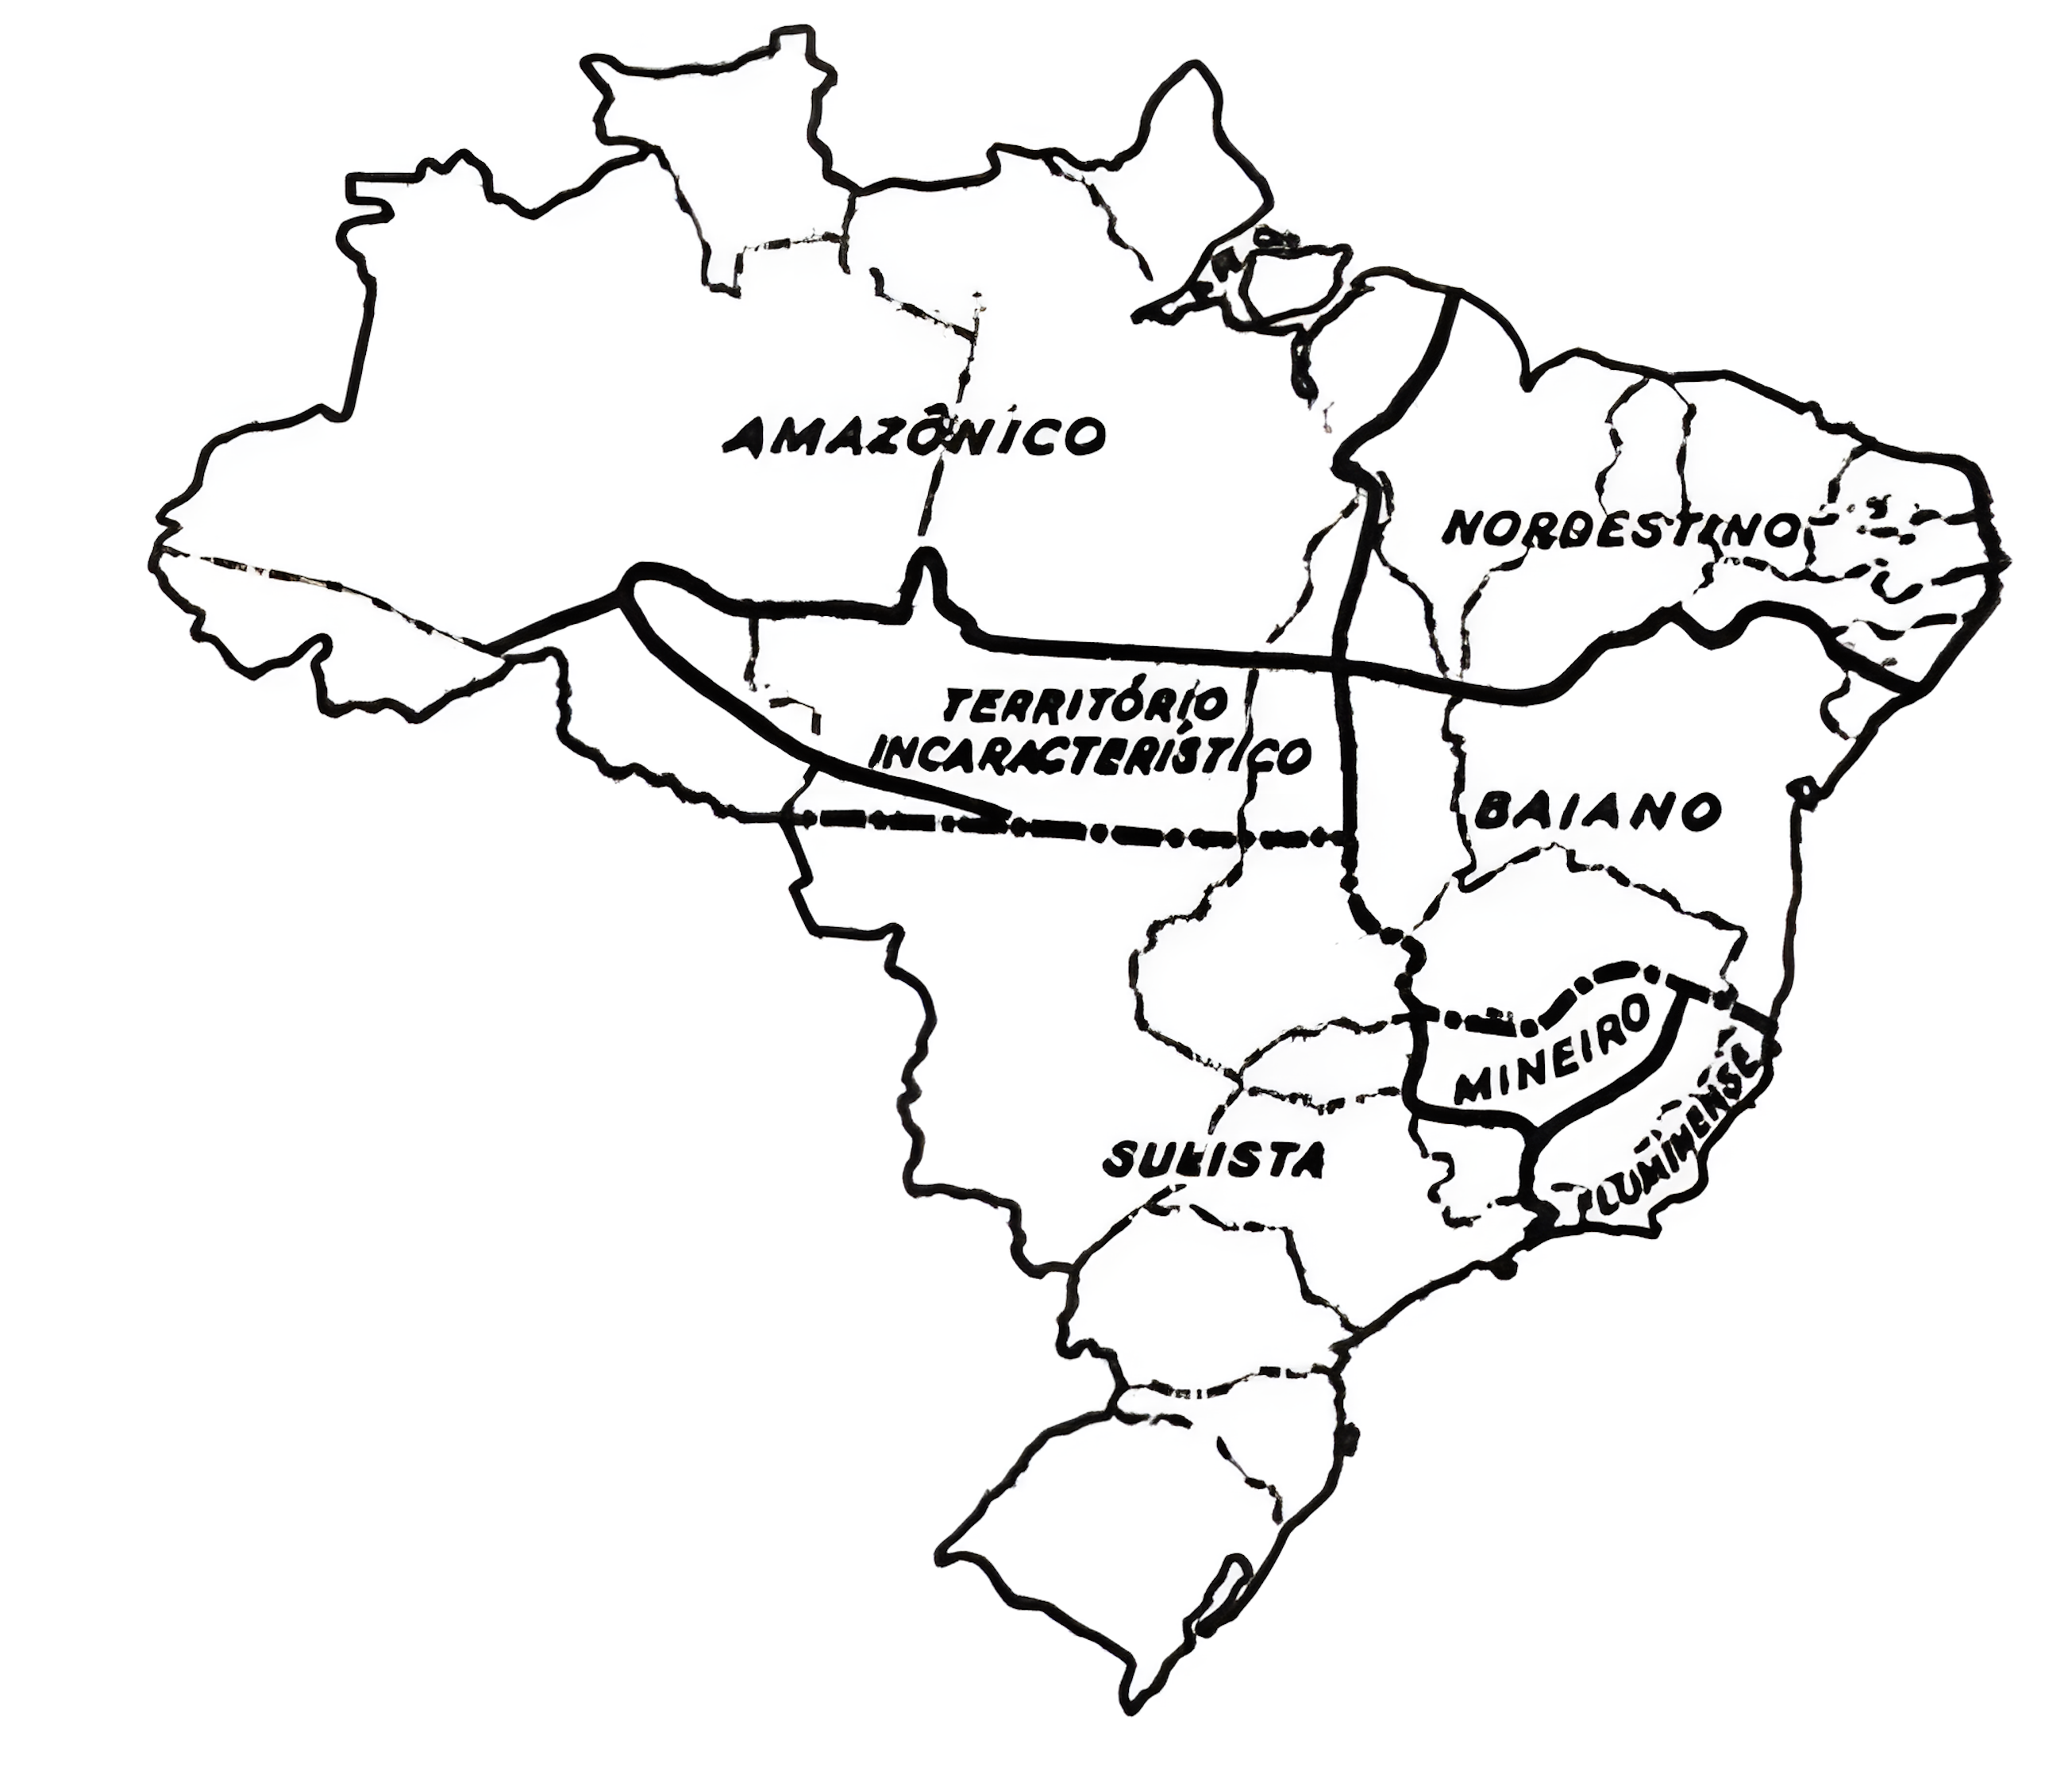
\includegraphics[width=0.75\linewidth]{images/mapa4x.png}
  \caption{Mapa da divisão dialetal de Nascentes (1950)}
  \label{fig:mapa1950}
\end{figure}
Um avanço significativo nos estudos dialetais brasileiros ocorreu com a criação do projeto Atlas Linguístico do Brasil (ALiB). Iniciado oficialmente em 1996, o ALiB congrega pesquisadores de diversas universidades com o objetivo de mapear e analisar a diversidade linguística do português falado no Brasil em seus múltiplos níveis (fonético-fonológico, morfossintático, léxico-semântico) \cite{cardoso2014alib, Aguilera2022}. Os volumes e artigos resultantes do ALiB têm fornecido um panorama muito mais detalhado e empiricamente fundamentado das variedades regionais.

Com base nos dados atualizados do Projeto ALiB e em outras pesquisas sociolinguísticas, Carlos Soares \cite{pagani2022}, em sua tese de doutorado, realizou um importante levantamento e sistematização, propondo uma cartografia dialetal que identifica 46 dialetos regionais no Brasil. Essa organização refina e expande consideravelmente os modelos anteriores, oferecendo um nível de granularidade mais adequado para aplicações que buscam sensibilidade às nuances locais. A Tabela \ref{tab:dialetos_pagani} apresenta um resumo dessa classificação, que serve de base para as análises subsequentes neste artigo. A precisão na representação dos 46 dialetos de Pagani e suas respectivas localizações é crucial, pois constitui o alicerce da classificação dialetal utilizada.



 % Início da Tabela 1 (Dialetos Brasileiros - Pagani 2022)
\begin{table}[ht]
\centering
\tiny
\setlength{\tabcolsep}{6pt}
\begin{tabular}{lll}
\hline
\textbf{Dialeto} & \textbf{UF(s)} & \textbf{Área / Localização} \\
\hline
\multicolumn{3}{l}{

\textbf{Região Norte e Amazônica}} \\ \hline
Nortista    & AC, AP, AM, PA, RO, RR, TO & Interior amazônico em geral \\
Manauara    & AM                         & Manaus e entorno urbano     \\
Belenense   & PA                         & Belém e Ilha de Marajó      \\
Rondoniense & RO                         & Porto Velho e interior      \\
Paraense    & PA                         & Interior sudeste e litoral  \\
\hline
\multicolumn{3}{l}{\textbf{Região Nordeste}} \\ \hline
Nordestino (genérico) & CE, PB, PE, BA, PI & Sertão semiárido do Nordeste       \\
Cearense              & CE                  & Fortaleza e Sertão Central–Cariri  \\
Maranhense            & MA                  & São Luís e Baixada Maranhense     \\
Paraibano             & PB                  & Litoral (João Pessoa) ao Cariri    \\
Pernambucano          & PE                  & Interior agreste-sertão (exc. Recife) \\
Recifense             & PE                  & Recife e Região Metropolitana      \\
Alagoano              & AL                  & Litoral de Maceió à Zona da Mata   \\
Sergipano             & SE                  & Estado inteiro (centro em Aracaju) \\
Teresinense           & PI                  & Capital Teresina                   \\
Sertanejo             & PI, BA, PE          & Faixa sertaneja semiárida          \\
\hline
\multicolumn{3}{l}{\textbf{Região Baiana}} \\ \hline
Baiano          & BA & Interior e litoral baiano em geral      \\
Soteropolitano  & BA & Salvador e Região Metropolitana         \\
Porto-Segurense & BA & Município de Porto Seguro               \\
Caravelense     & BA & Caravelas e litoral extremo sul         \\
Paulo-Afonsino  & BA & Cidade de Paulo Afonso, norte da BA     \\
\hline
\multicolumn{3}{l}{\textbf{Região Sudeste}} \\ \hline
Mineiro           & MG                     & Zona da Mata e Sul de Minas           \\
Belo-horizontino  & MG                     & Belo Horizonte e RM                   \\
Uberlandense      & MG                     & Uberlândia e Triângulo Mineiro        \\
Campo-Belense     & MG                     & Campo Belo, sul de Minas              \\
Carioca           & RJ                     & Rio de Janeiro e Baixada Fluminense   \\
Capixaba          & ES                     & Espírito Santo (todo o estado)        \\
Vitoriense        & ES                     & Ilha de Vitória e entorno             \\
Paulistano        & SP                     & Capital São Paulo e RM                \\
Paulista (interior)& SP                    & Centro-oeste e noroeste paulista      \\
Campineiro        & SP                     & Campinas e pólo tecnológico           \\
Piracicabano      & SP                     & Eixo Piracicaba–Limeira               \\
Santista          & SP                     & Baixada Santista                      \\
Sorocabano        & SP                     & Sorocaba e região                     \\
Botucatuense      & SP                     & Botucatu e serras centrais           \\
Bragantino        & SP                     & Bragança Paulista e Circuito das Águas\\
Capão-Bonitense   & SP                     & Capão Bonito e Vale do Paranapanema   \\
\hline
\multicolumn{3}{l}{\textbf{Região Sul}} \\ \hline
Sulista      & PR, SC                & Planaltos e planalto catarinense   \\
Paranaense   & PR                    & Interior do Paraná (exc. Curitiba) \\
Curitibano   & PR                    & Curitiba e RM                      \\
Cascavelense & PR                    & Cascavel e fronteira oeste         \\
Catarinense  & SC                    & Florianópolis e interior           \\
Gaúcho       & RS                    & Todo o Rio Grande do Sul           \\
\hline
\multicolumn{3}{l}{\textbf{Região Centro-Oeste}} \\ \hline
Goiano         & GO & Eixo Anápolis–Goiânia–Rio Verde  \\
Mato-Grossense & MT & Cuiabá e centro-sul de Mato Grosso \\
Brasiliense    & DF & Brasília e cidades-satélite        \\
\hline
\end{tabular}
\caption{Dialetos brasileiros e sua localização}
\label{tab:dialetos_pagani}
\end{table}
% fim da Tabela 1 (Dialetos Brasileiros - Pagani 2022)








\section{Distribuição Regional dos Dialetos}


A análise da Tabela \ref{tab:dialetos_pagani}, que sumariza os 46 dialetos identificados por Pagani (\citeyear{pagani2022}), revela uma distribuição heterogênea da diversidade linguística pelas cinco grandes regiões geográficas do Brasil. O gráfico de barras na  \ref{fig:dialetos-por-regiao} ilustra essa distribuição.


\begin{figure}
    \centering
    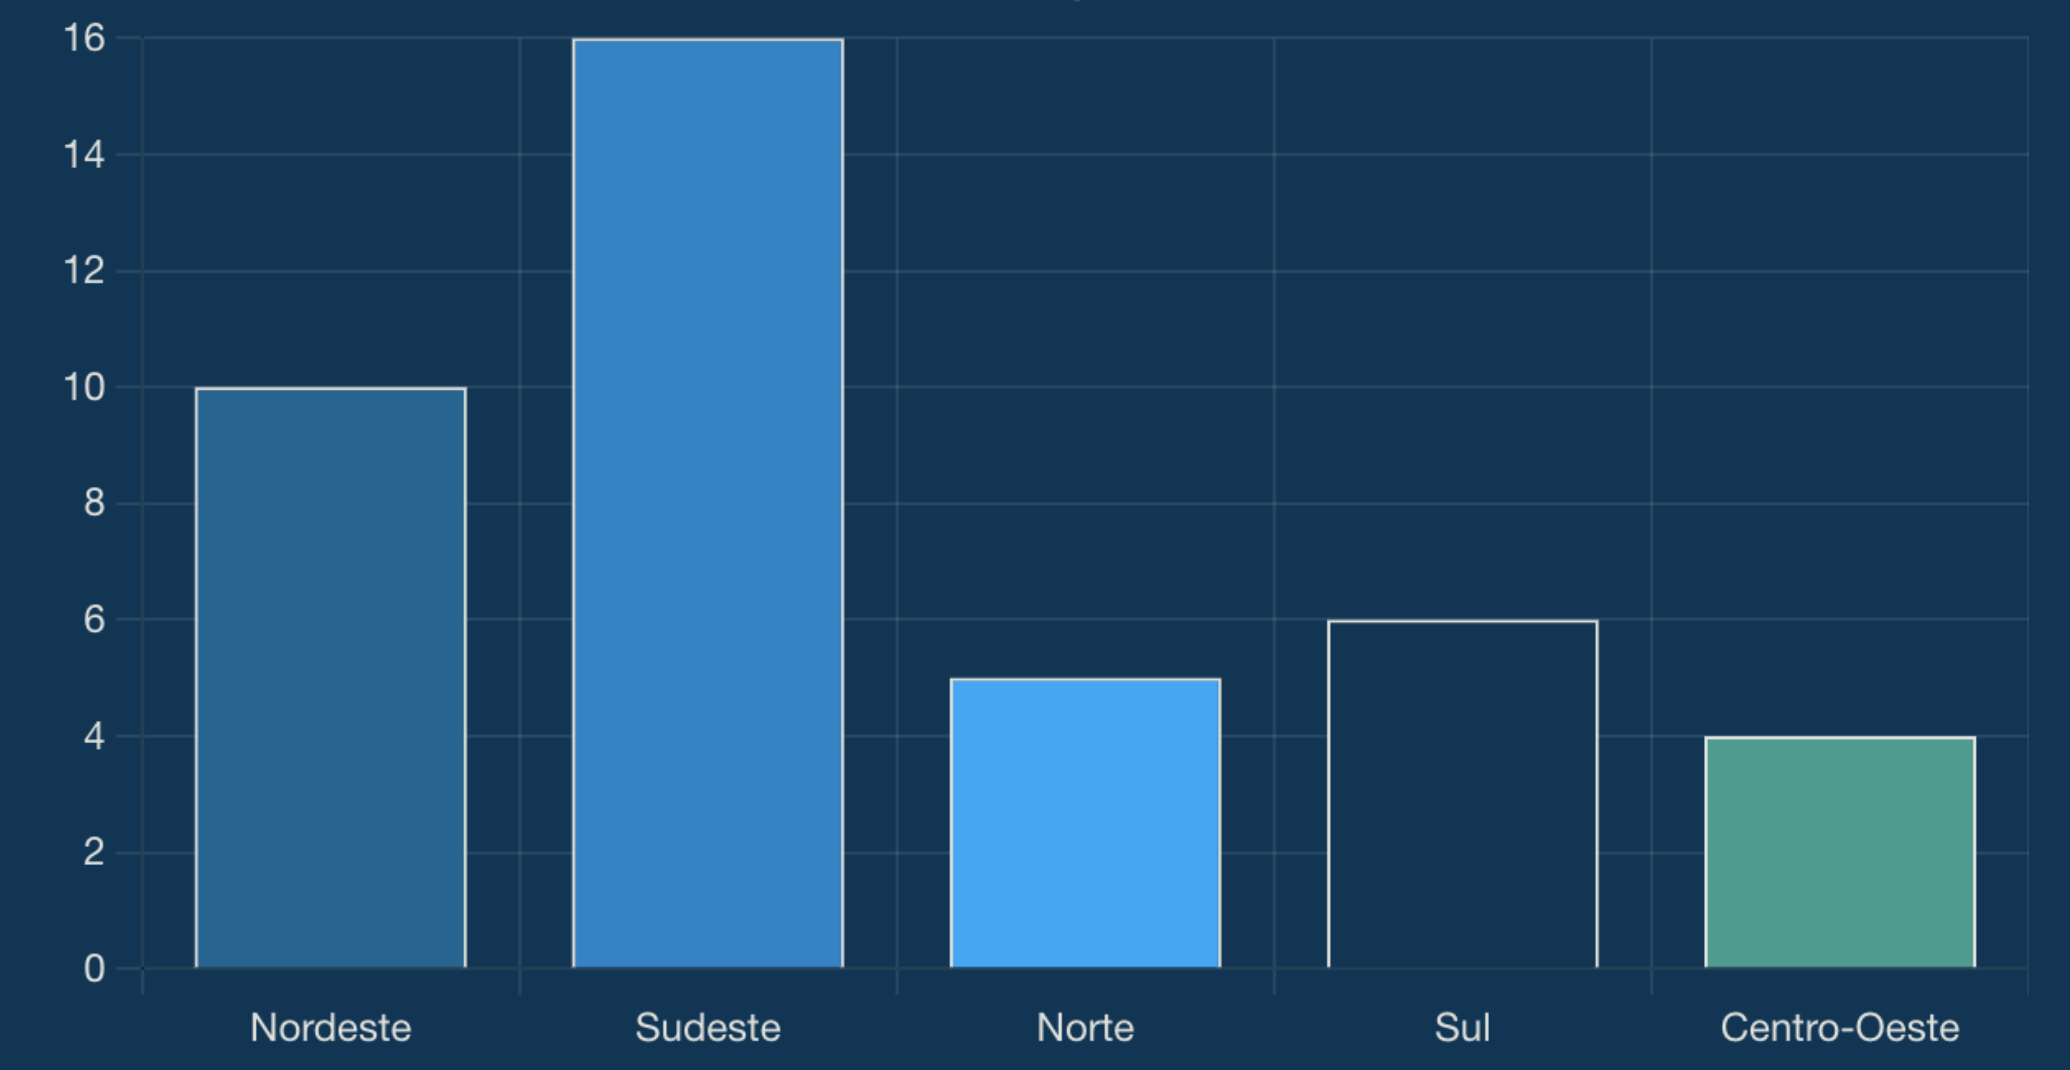
\includegraphics[width=0.75\linewidth]{images/grafico-dialetos-regiao.png}
    \caption{Dialetos por região}
    \label{fig:dialetos-por-regiao}
\end{figure}


Observa-se que a Região Sudeste desponta com o maior número de dialetos catalogados (16 variações), o que pode ser atribuído à sua complexidade demográfica, histórico de migrações internas e diversidade de processos de colonização e desenvolvimento econômico. Em seguida, a Região Nordeste (incluindo a subdivisão "Baiana" de Pagani) apresenta também uma riqueza considerável, com 10 dialetos listados. A Região Sul registra 6 dialetos, enquanto a Região Norte conta com 5. A Região Centro-Oeste, por sua vez, apresenta o menor número de dialetos principais identificados na classificação de Pagani (4 dialetos), refletindo, em parte, processos de ocupação mais recentes e vastas áreas com menor densidade populacional, embora também seja uma região de intenso contato linguístico devido a fluxos migratórios.

Essa visualização da concentração da diversidade dialetal em certas áreas e a relativa menor variação em outras (pelo menos no nível de granularidade da classificação de Pagani) é crucial. Ela destaca a necessidade de abordagens tecnológicas que não apenas reconheçam a existência de variação, mas que também sejam calibradas para as particularidades de cada macrorregião, e idealmente, para as sub-regiões dialetais.









\section{O plano de numeração e o mapa do DDD}


O Sistema de Discagem Direta à Distância (DDD) é um componente essencial da infraestrutura de telecomunicações brasileira. Trata-se de um plano de numeração telefônica implementado para permitir a realização de chamadas interurbanas de forma automática, sem a necessidade de intervenção de um operador humano. Sua implantação oficial ocorreu em 1969, sob a coordenação da então Embratel, e sua estrutura e regulamentação são hoje mantidas pela Agência Nacional de Telecomunicações (ANATEL), em conformidade com o Plano de Numeração Nacional \cite{anatel_pnb, felipe_embratel_2005}.

Cada código DDD corresponde a uma área geográfica específica, que pode abranger uma grande cidade e seu entorno metropolitano, ou um conjunto de municípios. Essa divisão forma um mapa administrativo-funcional que cobre a totalidade do território brasileiro. É fundamental ressaltar que a estruturação do sistema DDD foi pautada por critérios eminentemente técnicos, populacionais e administrativos, e não por considerações de natureza linguística. Consequentemente, as fronteiras das áreas DDD frequentemente não coincidem com os limites naturais das zonas dialetais, que são fruto de processos históricos, sociais e culturais de longa duração.

Apesar dessa desvinculação original, a ampla disseminação do sistema DDD, sua estabilidade relativa ao longo do tempo e, crucialmente, a familiaridade da população com seus códigos, tornam-no um candidato pragmático para servir como uma camada inicial de referência geográfica no mapeamento de dialetos para fins tecnológicos. A ANATEL disponibiliza informações sobre o plano de numeração em seus canais oficiais, sendo importante consultar os dados mais recentes para garantir a precisão de qualquer análise baseada nesses códigos \cite{anatel_pnb}. A \ref{fig:mapa-ddd} apresenta uma representação visual do mapa de códigos DDD no Brasil. A utilização da versão mais atualizada deste mapa e dos dados de abrangência dos DDDs é uma premissa metodológica para a validade da associação com os dialetos.


\cite{anatel_pnb}.
\begin{figure}[ht]
  \centering
  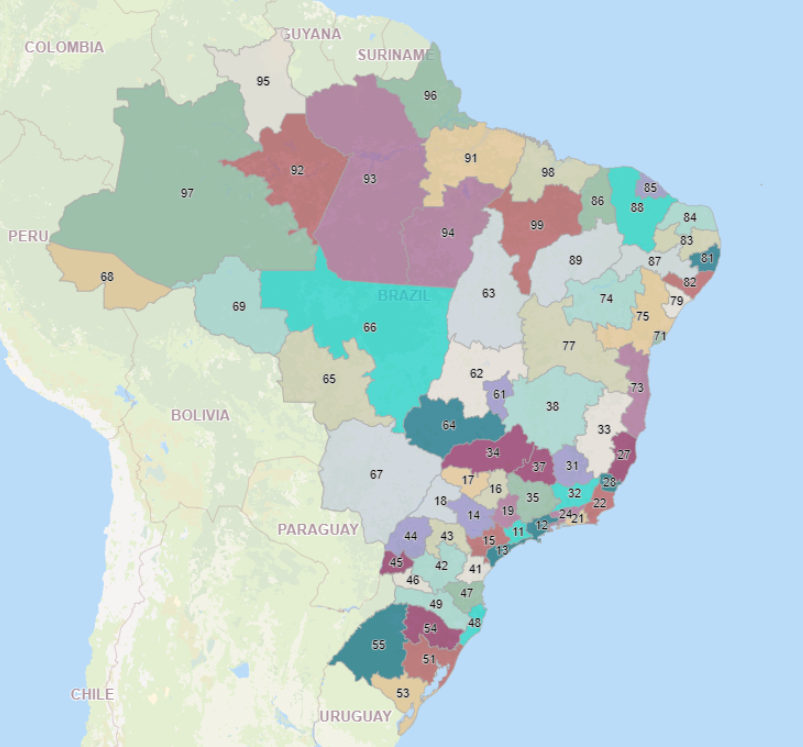
\includegraphics[width=\linewidth]{images/mapa_ddd_brasil.png}
  \caption{Mapa do Plano de Numeração Brasileiro (DDDs)}
  \label{fig:mapa-ddd}
\end{figure}

\section{Associação entre DDDs e Dialetos}


A etapa crucial desta proposta é o estabelecimento de uma correspondência entre os códigos DDD e as zonas dialetais brasileiras, conforme a classificação de Pagani (\citeyear{pagani2022}). A Tabela \ref{tab:ddd-dialeto-todas} apresenta o resultado dessa associação, que busca aproximar os limites administrativos consolidados pelo sistema DDD da realidade sociolinguística do país. É importante notar que esta tabela representa uma aproximação e está sujeita às limitações inerentes ao cruzamento de dois sistemas de zoneamento com naturezas e propósitos distintos.

A análise dessa associação revela diferentes cenários de correspondência:
\begin{enumerate}
    \item \textbf{Correspondência direta:} Casos em que um código DDD parece alinhar-se de forma relativamente clara com a área de ocorrência principal de um dialeto específico. Por exemplo, o DDD 71 (Salvador e Região Metropolitana) com o dialeto Soteropolitano, ou o DDD 41 (Curitiba e Região Metropolitana) com o dialeto Curitibano.
    \item \textbf{Múltiplos DDDs para um mesmo dialeto:} Situações em que um dialeto com ampla extensão geográfica é coberto por diversos códigos DDD. É o caso do dialeto Paulista (interior), que se espalha por DDDs como 12, 14, 16, 17 e 18, ou do dialeto Gaúcho, abrangendo os DDDs 51, 53, 54 e 55.
    \item \textbf{DDDs que abrangem múltiplos dialetos:} Ocorrências em que um único código DDD engloba áreas onde diferentes dialetos são predominantes ou coexistem. Por exemplo, o DDD 73 na Bahia, que cobre áreas do dialeto Baiano e do Porto-Segurense, ou o DDD 35 em Minas Gerais, que inclui regiões do dialeto Mineiro e do Campo-Belense.
    \item \textbf{Dialetos sem DDD específico ou com representação parcial:} Casos em que dialetos com menor extensão territorial ou localizados em áreas de transição não possuem um DDD exclusivo, estando inseridos em um código de área mais amplo. Exemplos incluem o dialeto Caravelense (contido no DDD 73) ou o Botucatuense (no DDD 14).
\end{enumerate}

Essas sobreposições e lacunas são reflexos diretos das divergências fundamentais entre os critérios de formação dos dialetos e de estabelecimento dos DDDs. Dialetos são formados por processos históricos, socioculturais e geográficos complexos, evoluindo organicamente ao longo de gerações e apresentando, frequentemente, fronteiras graduais e porosas (isoglossas). Em contraste, os DDDs são definidos por critérios administrativos, técnicos e demográficos, com fronteiras rígidas e bem delimitadas, geralmente acompanhando limites político-administrativos de municípios ou agrupamentos deles. Adicionalmente, a granularidade e a escala dos dois sistemas são distintas: os dialetos podem variar significativamente mesmo dentro de um mesmo estado ou município, enquanto os DDDs tendem a agrupar grandes áreas sob um único código, especialmente em regiões menos densamente povoadas.



\begin{table}[ht]
  \centering
  \tiny
  \setlength{\tabcolsep}{6pt}
  \begin{tabular}{llll}
    \toprule
    \textbf{DDD} & \textbf{Estados} & \textbf{Dialeto Principal} & \textbf{Subdialetos / Observações} \\
    \midrule
    \multicolumn{4}{l}{\textbf{Região Norte}} \\ 
    91 & PA      & Belenense             & Abrange a capital Belém e região metropolitana \\
    92 & AM      & Manauara              & Centrado em Manaus e entorno                  \\
    93 & PA      & Paraense              & Interior do Pará (oeste)                      \\
    94 & PA      & Paraense              & Interior do Pará (sudeste)                    \\
    95 & RR      & Nortista              & Variante roraimense                           \\
    96 & AP      & Nortista              & Variante amapaense                            \\
    97 & AM      & Nortista              & Interior do Amazonas                          \\
    98 & MA      & Maranhense            & São Luís e norte do estado                    \\
    99 & MA      & Maranhense/Nordestino & Sul do Maranhão com influências nordestinas   \\
    \midrule
    \multicolumn{4}{l}{\textbf{Região Nordeste}} \\ 
    71 & BA & Soteropolitano          & Salvador e Região Metropolitana          \\
    73 & BA & Baiano/Porto-Segurense  & Litoral sul da Bahia                     \\
    74 & BA & Baiano                  & Sertão baiano                            \\
    75 & BA & Baiano                  & Região central da Bahia                  \\
    77 & BA & Baiano/Sertanejo        & Extremo oeste baiano                     \\
    79 & SE & Sergipano               & Todo o estado de Sergipe                 \\
    81 & PE & Recifense               & Recife e Região Metropolitana            \\
    82 & AL & Alagoano                & Todo o estado de Alagoas                 \\
    83 & PB & Paraibano               & Todo o estado da Paraíba                 \\
    84 & RN & Nordestino              & Variante potiguar                        \\
    85 & CE & Cearense                & Fortaleza e região metropolitana         \\
    86 & PI & Teresinense             & Capital e centro-norte do Piauí          \\
    87 & PE & Pernambucano            & Interior de Pernambuco                   \\
    88 & CE & Cearense                & Interior do Ceará                        \\
    89 & PI & Nordestino/Sertanejo    & Sul do Piauí                             \\
    \midrule
    \multicolumn{4}{l}{\textbf{Região Centro-Oeste}} \\ 
    61 & DF/GO & Brasiliense       & Brasília, entorno e nordeste goiano   \\
    62 & GO    & Goiano            & Goiânia e centro de Goiás             \\
    63 & TO    & Nortista          & Com influências do dialeto nordestino \\
    64 & GO    & Goiano            & Sul de Goiás                          \\
    65 & MT    & Mato-Grossense    & Cuiabá e centro-sul de MT             \\
    66 & MT    & Mato-Grossense    & Norte e leste de MT                   \\
    67 & MS    & Sulista           & Com influências do dialeto paranaense \\
    68 & AC    & Nortista          & Variante acreana                      \\
    69 & RO    & Rondoniense       & Todo o estado de Rondônia             \\
    \midrule
    \multicolumn{4}{l}{\textbf{Região Sudeste}} \\ 
    11 & SP & Paulistano            & São Paulo e Região Metropolitana        \\
    12 & SP & Paulista (interior)   & Vale do Paraíba                         \\
    13 & SP & Santista              & Baixada Santista                        \\
    14 & SP & Paulista (interior)   & Bauru e região                          \\
    15 & SP & Sorocabano            & Sorocaba e região                       \\
    16 & SP & Paulista (interior)   & Ribeirão Preto e região                 \\
    17 & SP & Paulista (interior)   & São José do Rio Preto e noroeste        \\
    18 & SP & Paulista (interior)   & Presidente Prudente e oeste paulista    \\
    19 & SP & Campineiro            & Campinas e região                       \\
    21 & RJ & Carioca               & Rio de Janeiro e Região Metropolitana    \\
    22 & RJ & Fluminense            & Norte e noroeste fluminense             \\
    24 & RJ & Fluminense            & Região serrana do RJ                    \\
    27 & ES & Capixaba/Vitoriense   & Grande Vitória                          \\
    28 & ES & Capixaba              & Sul do Espírito Santo                   \\
    31 & MG & Belo-horizontino      & Belo Horizonte e Região Metropolitana    \\
    32 & MG & Mineiro               & Zona da Mata mineira                    \\
    33 & MG & Mineiro               & Vale do Jequitinhonha e Mucuri          \\
    34 & MG & Uberlandense          & Triângulo Mineiro                       \\
    35 & MG & Mineiro/Campo-Belense & Sul de Minas                            \\
    37 & MG & Mineiro               & Centro-oeste de Minas                   \\
    38 & MG & Mineiro               & Norte de Minas                          \\
    \midrule
    \multicolumn{4}{l}{\textbf{Região Sul}} \\ 
    41 & PR & Curitibano        & Curitiba e Região Metropolitana     \\
    42 & PR & Paranaense        & Centro-sul do Paraná                \\
    43 & PR & Paranaense        & Norte do Paraná                     \\
    44 & PR & Paranaense        & Noroeste do Paraná                  \\
    45 & PR & Cascavelense      & Oeste do Paraná                     \\
    46 & PR & Paranaense        & Sudoeste do Paraná                  \\
    47 & SC & Catarinense       & Norte de Santa Catarina             \\
    48 & SC & Catarinense       & Grande Florianópolis e litoral      \\
    49 & SC & Catarinense       & Oeste de Santa Catarina             \\
    51 & RS & Gaúcho            & Porto Alegre e região metropolitana \\
    53 & RS & Gaúcho            & Sul do Rio Grande do Sul            \\
    54 & RS & Gaúcho            & Serra gaúcha                        \\
    55 & RS & Gaúcho            & Oeste e noroeste do Rio Grande do Sul \\
    \bottomrule
  \end{tabular}
  \caption{Tabela de Associação DDD–Dialeto (todas as regiões)}
  \label{tab:ddd-dialeto-todas}
\end{table}











\section{Análise Crítica: Limitações e Oportunidades da Abordagem}

A proposta de utilizar o sistema de Discagem Direta à Distância (DDD) como referência para o mapeamento de dialetos brasileiros, embora pragmática, necessita de uma análise crítica que pondere suas limitações e as oportunidades que oferece para o desenvolvimento de tecnologias linguisticamente sensíveis.

\subsection{Limitações}


As principais limitações desta abordagem derivam da natureza fundamentalmente distinta entre a organização administrativa dos DDDs e a complexa realidade sociolinguística.

\textbf{Impacto da Mobilidade Populacional:} Um dos desafios mais significativos é a intensa mobilidade populacional no Brasil. Dados do Censo Demográfico de 2010 do IBGE indicavam que aproximadamente 36,9\% da população brasileira residia em municípios diferentes de seus locais de nascimento \cite{noauthor_ibge_nodate}. Essa dinâmica migratória expressiva significa que uma parcela considerável de indivíduos pode utilizar um DDD de uma determinada região, mas manter o sotaque e as características linguísticas de sua região de origem, ou mesmo desenvolver formas híbridas. A \ref{fig:gradico-migracoes} ilustra a relevância desse fenômeno com base nos dados disponíveis. Essa mobilidade introduz um ruído considerável na correlação direta entre DDD e dialeto falado pelo usuário individual.


\begin{figure}
    \centering
    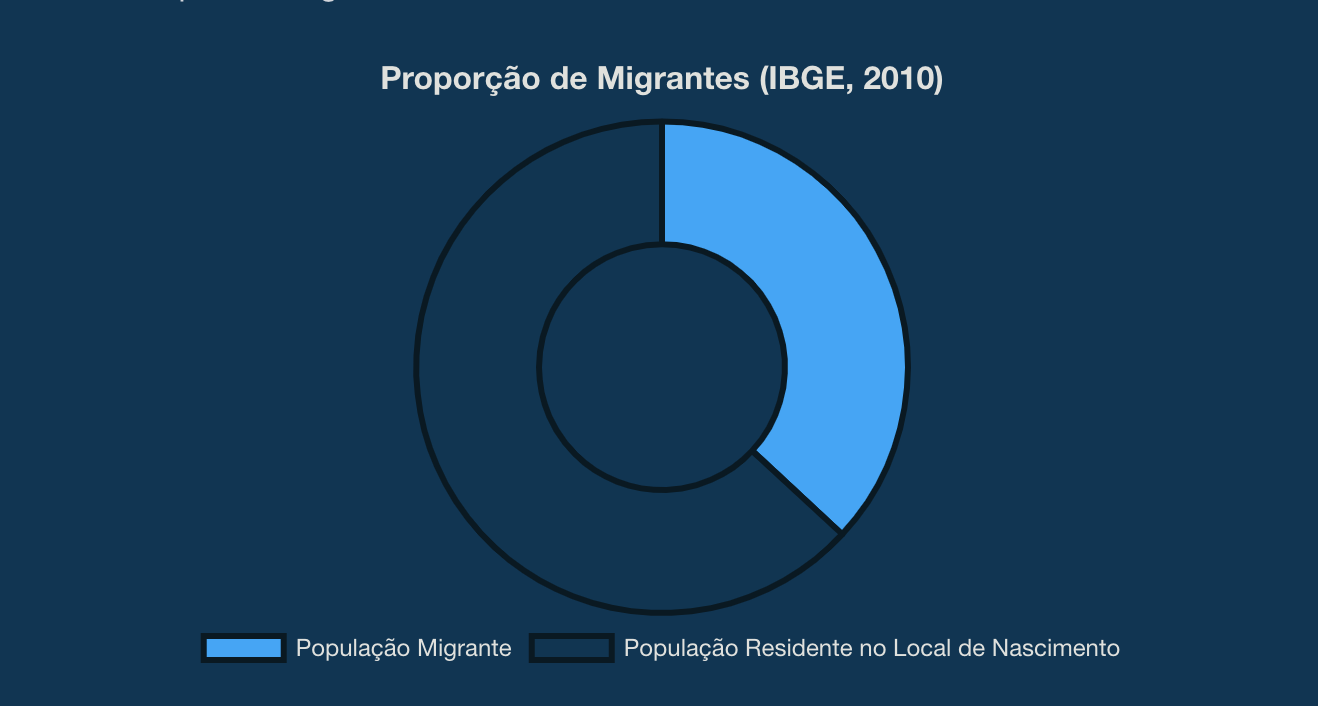
\includegraphics[width=0.8\linewidth]{images/grafico-dos-migrantes.png}
    \caption{Proporção de Migrantes Internos no Brasil}
    \label{fig:gradico-migracoes}
\end{figure}



\textbf{Simplificação Excessiva:} O sistema DDD, por sua concepção administrativa, agrupa, por vezes, áreas geograficamente extensas e linguisticamente heterogêneas sob um mesmo código. Isso leva a uma simplificação drástica da complexidade dialetal real, onde múltiplas variantes e nuances podem coexistir dentro de uma única área DDD.

\textbf{Distorções Regionais:} A granularidade dos DDDs não é uniforme em todo o território nacional. Regiões mais populosas e economicamente desenvolvidas tendem a ter uma maior subdivisão de códigos DDD, enquanto vastas áreas menos povoadas podem ser cobertas por um único código. Essa distribuição desigual pode distorcer a representação da diversidade dialetal, que não necessariamente segue a mesma lógica demográfica ou econômica.

\textbf{Fronteiras Artificiais:} As fronteiras entre as áreas DDD são definidas por limites municipais e estaduais, que são demarcações político-administrativas. As fronteiras dialetais, por outro lado, são fenômenos socioculturais que raramente coincidem com essas divisões estanques. As isoglossas, linhas imaginárias que marcam os limites de ocorrência de determinados traços linguísticos, frequentemente cruzam fronteiras administrativas, criando zonas de transição e continuidade que o sistema DDD não captura.

\textbf{Ausência de Representação de Microdialetos e Variedades de Contato:} O sistema DDD, em sua escala macrorregional, não tem capacidade para representar microdialetos, como os falados em comunidades específicas (quilombolas, indígenas que também falam português, comunidades de imigrantes mantenedoras de variedades próprias do português), nem as complexas variações que surgem em áreas de intenso contato linguístico. Essas formas, embora minoritárias em termos de número de falantes, possuem grande significado cultural e identitário.

A consideração desses fatores não invalida a proposta, mas sublinha a necessidade de se compreender o mapeamento DDD-dialeto como uma primeira aproximação, um ponto de partida que pode requerer refinamentos e a integração de outras fontes de informação (como autodeclaração do usuário ou dados de geolocalização mais precisos, quando eticamente permissível e tecnicamente viável) para aplicações que exijam maior acurácia individual.










\section{oportunidades}
Apesar das limitações expostas, a utilização do mapa de DDDs como referência para o mapeamento dos dialetos brasileiros apresenta vantagens significativas, especialmente sob uma perspectiva pragmática e de escalabilidade tecnológica.

\textbf{Praticidade e Reconhecimento:} O sistema de DDD é amplamente conhecido e utilizado pela população brasileira em seu cotidiano. Essa familiaridade pode facilitar a implementação e a aceitação de tecnologias que utilizem essa divisão como base para adaptação linguística, tornando a interação mais intuitiva para o usuário.

\textbf{Infraestrutura Existente:} As tecnologias de telecomunicação, incluindo telefonia móvel e fixa, já operam sobre a base do sistema DDD. Isso significa que existe uma infraestrutura consolidada que pode ser aproveitada para a implementação de soluções que considerem variações linguísticas regionais, sem a necessidade de criar do zero um novo sistema de identificação geográfica para esse fim.

\textbf{Correlação Parcial Significativa:} Embora as fronteiras não sejam coincidentes, existe, em muitos casos, uma correlação parcial, porém significativa, entre as áreas de DDD e as grandes zonas dialetais, especialmente em um nível macrorregional. Para muitas aplicações, essa aproximação pode ser suficiente para um primeiro nível de personalização linguística. O valor reside em ser uma heurística "boa o suficiente" em cenários onde dados mais granulares são inexistentes ou de difícil obtenção.

\textbf{Escalabilidade Tecnológica:} A estrutura do sistema DDD é particularmente útil para aplicações que utilizam o número de telefone como forma primária de identificação ou contato, como é o caso de serviços baseados em WhatsApp, Telegram, Signal, SMS, chatbots e sistemas de atendimento automatizado por voz (URA). Por estar integrada à lógica de numeração nacional e ser amplamente reconhecida, essa estrutura oferece um ponto de partida escalável para o desenvolvimento de tecnologias adaptativas. Essas tecnologias podem, então, ser progressivamente refinadas com base em dados reais de uso, feedback dos usuários e, quando aplicável, informações de localização mais precisas fornecidas com consentimento.

Essas oportunidades sugerem que a abordagem DDD-dialeto, se implementada com consciência de suas limitações e com mecanismos para aprimoramento contínuo, pode representar um avanço importante na criação de tecnologias mais inclusivas e culturalmente relevantes para o contexto brasileiro.

\section{Aplicações Tecnológicas e Implicações Socioculturais}


A proposta de utilizar o sistema de Discagem Direta à Distância (DDD) como referência para o mapeamento dos dialetos brasileiros abre um leque de possibilidades para o desenvolvimento de tecnologias assistivas e para o fortalecimento da comunicação, especialmente em contextos que exigem maior sensibilidade cultural e linguística, como o rural. Ao alavancar uma estrutura já consolidada e familiar à população, integrada a plataformas de comunicação amplamente utilizadas (como WhatsApp, Telegram, Signal, chamadas automáticas, chatbots e SMS), torna-se viável criar soluções mais acessíveis, culturalmente pertinentes e com potencial de escalabilidade.

Entre as principais aplicações potenciais, destacam-se:
\begin{enumerate}
    \item \textbf{Assistentes Virtuais Regionalmente Adaptados:} Desenvolvimento de agentes conversacionais (chatbots, voicebots) que ajustem seu vocabulário, prosódia (entonação, ritmo) e construções sintáticas com base no perfil dialetal predominante associado ao DDD do usuário. Isso pode favorecer maior compreensão, naturalidade na interação e sentimento de identificação com a tecnologia, sendo particularmente relevante em serviços de saúde, educação, atendimento ao cidadão e suporte técnico.
    \item \textbf{Sintetização de Voz (TTS) Inclusiva:} Aprimoramento de sistemas de Text-to-Speech (processo de sintetizar a fala humana a partir do texto escrito) para gerar fala com maior fidelidade aos sotaques e variações locais. Em vez de uma voz padrão única, muitas vezes percebida como distante ou artificial, poderiam ser oferecidas opções de vozes regionais, promovendo maior acessibilidade e conforto para populações com padrões linguísticos distintos do português padrão veiculado nos grandes meios de comunicação.
    \item \textbf{Interfaces de ATER Digital Culturalmente Sensíveis:} Criação de plataformas digitais de Assistência Técnica e Extensão Rural (ATER) que utilizem uma linguagem próxima à do público-alvo (agricultores familiares, comunidades tradicionais). Isso inclui vocabulário técnico adaptado, exemplos regionalizados, e a possibilidade de interação por voz utilizando comandos e formulações mais intuitivas para o falante local. Tal abordagem pode facilitar a compreensão de orientações técnicas, o envio de dúvidas e o compartilhamento de conhecimentos.
    \item \textbf{Ferramentas de Mediação Linguística Interdialetal:} Desenvolvimento de aplicativos ou funcionalidades que atuem como "pontes" comunicativas entre falantes de diferentes variedades do português brasileiro. Seriam úteis em contextos de migração interna, feiras e eventos agrícolas de abrangência nacional, turismo regional, programas de educação de jovens e adultos com turmas heterogêneas, ou em serviços públicos que atendem pessoas de diversas origens regionais.
    \item \textbf{Materiais Educativos Linguisticamente Inclusivos:} Produção de conteúdos didáticos digitais (vídeos, áudios, jogos educativos, aplicativos) que levem em consideração as formas regionais de falar. Isso não apenas promove o respeito à diversidade linguística e cultural desde cedo, mas também pode tornar o processo de aprendizagem mais significativo e eficaz, sobretudo em contextos de alfabetização e formação técnica rural, onde a língua padrão pode representar uma barreira adicional.
    \item \textbf{Sistemas Regionalizados de Alerta e Informação:} Implantação de serviços automatizados para envio de informações relevantes (alertas meteorológicos, comunicados sanitários, instruções sobre práticas agrícolas, informações de utilidade pública) em linguagem acessível e com sotaque local, aproveitando bases de contatos organizadas por DDD e região.
\end{enumerate}

Essas aplicações encontram forte ressonância nos princípios do dialogismo de Mikhail Bakhtin e na pedagogia libertadora de Paulo Freire. Como destaca Bakhtin, a linguagem é inerentemente polifônica, e cada voz social carrega consigo uma perspectiva única \cite{bakhtin1997estetica}. Tecnologias que reconhecem e se adaptam a essa polifonia estão, em essência, validando essas múltiplas perspectivas. Paulo (\citeyear{freire2005pedagogia}), por sua vez, enfatiza que a comunicação autêntica não se limita à transmissão unilateral de informações, mas se constrói no encontro de vozes e saberes, exigindo escuta ativa e respeito aos modos de expressão populares.

No contexto da comunicação rural, essa abordagem adquire relevância ainda maior diante dos desafios persistentes de conectividade, níveis de escolaridade e desigualdades sociolinguísticas. Como apontado por estudos sobre ATER Digital (\cite{parra2022ater}), a tecnologia deve ir além de uma visão instrumental, sendo concebida como um espaço de mediação social. Nesse espaço, o respeito à linguagem do agricultor e da agricultora é condição fundamental para o estabelecimento do diálogo, para o seu protagonismo e para a efetividade das políticas públicas e iniciativas de desenvolvimento.


\section{Conclusão}


Este artigo investigou e propôs a utilização do sistema de Discagem Direta à Distância (DDD) como um mapa de referência inicial para a identificação e organização de falantes segundo os dialetos brasileiros. O objetivo primordial que norteou esta análise foi o de subsidiar o desenvolvimento de tecnologias assistivas que sejam linguisticamente sensíveis e adaptativas à vasta pluralidade de falares do Brasil.

A análise empreendida demonstrou que, embora a correlação entre as áreas de DDD e as zonas dialetais apresente limitações – notadamente devido à mobilidade populacional, à simplificação da complexidade dialetal inerente ao sistema DDD e às fronteiras administrativas que não espelham as fronteiras linguísticas naturais – existem também correlações parciais significativas e, crucialmente, uma infraestrutura prática e já estabelecida. Os resultados indicam que o sistema de DDD, mesmo com seus desafios, oferece um ponto de partida viável e pragmático para o avanço de tecnologias que buscam respeitar e valorizar a diversidade linguística nacional.

Assim, o estudo responde afirmativamente à possibilidade de utilizar os códigos DDD como uma camada inicial para inferência de perfil dialetal regional. A principal contribuição deste trabalho reside em pavimentar um caminho metodológico e conceitual para a criação de ferramentas tecnológicas que não apenas reconheçam passivamente, mas que celebrem ativamente os sotaques e falares locais. Ao fazer isso, promove-se não somente a inclusão digital, facilitando o acesso e a interação de um espectro mais amplo da população, mas também o respeito às múltiplas identidades culturais que compõem o mosaico brasileiro.

As implicações práticas desta proposta são vastas e promissoras. Elas incluem o desenvolvimento de assistentes virtuais regionalmente adaptados, sistemas de sintetização de voz mais inclusivos e representativos, interfaces de Assistência Técnica e Extensão Rural (ATER) Digital que "falem a língua" do agricultor, aplicativos de mediação linguística interdialetal e materiais educativos que reflitam e valorizem a riqueza dos falares regionais. Tais aplicações encontram profundo eco nos princípios do dialogismo de Bakhtin e na pedagogia libertadora de Paulo Freire, que concebem a comunicação como um encontro genuíno de vozes e saberes e que valorizam as variações linguísticas como expressões autênticas da identidade cultural e da vivência social \cite{bakhtin1997estetica, freire2005pedagogia, freire2013extensao}.

Como próximos passos, sugere-se a continuidade desta pesquisa através do refinamento do mapa de associação DDD-dialeto, possivelmente com a incorporação de dados mais granulares sobre a distribuição populacional e fluxos migratórios. A exploração de técnicas de aprendizado de máquina para uma identificação dialetal mais dinâmica e precisa, que possa ir além da simples correlação com o DDD (por exemplo, analisando características da própria fala do usuário, com seu consentimento), também se apresenta como um campo fértil. Adicionalmente, estudos de usabilidade e impacto sobre a eficácia e aceitação de tecnologias linguisticamente adaptadas por diferentes comunidades de falantes seriam de grande valia.

Finalizando, a utilização criteriosa e consciente do mapa de DDDs como ponto de partida para o mapeamento dos dialetos brasileiros configura um avanço significativo rumo ao desenvolvimento de tecnologias que efetivamente abracem a diversidade cultural e linguística do país. Esta abordagem, ao alinhar-se com perspectivas teóricas que prezam pelo diálogo, pela valorização identitária e pela comunicação libertadora, não só enriquece o campo tecnológico, mas também contribui ativamente para a construção de uma sociedade digital mais justa, inclusiva e genuinamente brasileira. Encoraja-se, portanto, a colaboração interdisciplinar entre linguistas, engenheiros de software, designers de interação e formuladores de políticas públicas para que o potencial aqui delineado possa ser plenamente realizado, transformando a tecnologia em uma aliada da diversidade.
